\section{Proofs: the constrained style}
\label{sec:proofs}

% ---------------------------------------------------------------------------
% Fitch-style proof drawing macros (local to this chapter, \prf prefix).
%   \prfstart                          origin node (p0); call first
%   \prfline{name}{prev}{depth}{num}{text}{rule}
%        one proof line, placed under node {prev}; depth 0 = outside every
%        subproof; the rule label sits right-aligned in its own column
%   \prfscope{first}{last}{depth}{bar}
%        vertical scope bar from line {first} to line {last} at {depth},
%        plus the short horizontal "assumption" bar under {first}
% ---------------------------------------------------------------------------
\newcommand{\prfgap}{0.5cm}
\newcommand{\prfstart}{\node[inner sep=0pt,minimum size=0pt] (p0) at (0,0) {};}
\newcommand{\prfline}[6]{%
  \node[anchor=north west,inner sep=2pt,font=\small,align=flush left,
        text width=\dimexpr 10.9cm-#3\dimexpr\prfgap\relax\relax]
    (#1t) at ($(0,0 |- #2.south)+(0.7cm+#3*\prfgap,-1.2pt)$) {#5};
  \node[anchor=north east,inner sep=2pt,font=\small,align=flush right,text width=4.3cm]
    (#1r) at ($(0,0 |- #1t.north)+(16.3cm,0)$) {#6};
  \node[anchor=north west,inner sep=2pt,font=\small] at (0,0 |- #1t.north) {#4};
  \node[fit=(#1t)(#1r),inner sep=0pt] (#1) {};}
\newcommand{\prfscope}[4]{%
  \draw ($(0,0 |- #1.north)+(0.7cm+#3*\prfgap-0.16cm,-1.2pt)$)
     -- ($(0,0 |- #2.south)+(0.7cm+#3*\prfgap-0.16cm,1.2pt)$);
  \draw ($(0,0 |- #1t.south)+(0.7cm+#3*\prfgap-0.16cm,0)$) -- ++(#4,0);}
\newcommand{\prfqed}{\ $\mdlgwhtsquare$}

This is the part of Test 1 where points actually get lost. Computing $A-B$ or filling in a truth table is mechanical. A constrained proof isn't: you have to pick a move, justify it with exactly the right rule, and not take a step that only \emph{feels} valid. The good news is that the moves are few and the choice of move is almost always forced by what the goal looks like. This chapter is about learning to see that.

Everything here comes from notes \S3.1--3.13 and the subset material in \S2.5.1. Every claim in this chapter was written fresh for this guide, and each was checked by brute force over all subsets of $\{0,1,2,3\}$.

\subsection{What counts as a proof in this course}

A proof is a chain of reasoning where every step follows logically from things you already have. That's it. How much detail you show, and what format you use, varies a lot, and the notes sort proofs into three kinds:

\begin{itemize}
  \item A \emph{formal proof} uses a fixed, small set of logical rules and a rigid format, like source code for an argument. Logicians write these when they're studying logic itself or feeding proofs to a computer.
  \item An \emph{informal proof} is everything else: textbook proofs, papers, the stuff on a whiteboard. Still airtight, but any valid rule is allowed and the writer decides how much detail the reader needs. Informal doesn't mean sloppy.
  \item A \emph{constrained proof} is the middle ground this course uses for now. It's written in ordinary English sentences, but you may only use the rules and definitions on the list you're given, at most one rule (plus at most one definition) per line, and you must name what you used.
\end{itemize}

Why bother with the constrained style? Because it makes every step checkable. In an informal proof, ``clearly $x\notin B$'' can hide a broken inference. In a constrained proof, that line has to carry a rule name, and the grader can hold it up against the rule's exact wording. So can you.

Here's the mental model that makes the rest of this chapter click. Think of a proof as a game. The \emph{goal} (what you're trying to show) has a shape, and that shape tells you your opening move. The facts you're \emph{holding} also have shapes, and they tell you what you can do next. You win when what you hold matches the goal.

\subsection{The toolkit}

\subsubsection{Five definitions}

For set proofs you'll get these definitions, and only these. Each one turns a statement about sets into a statement about a single member $x$, which is what makes the rules usable.

\begin{center}
\begin{tabularx}{\linewidth}{@{}l>{\raggedright\arraybackslash}p{6.6cm}L@{}}
\toprule
\textbf{Cite as} & \textbf{Definition} & \textbf{Logic inside it}\\
\midrule
def.\ of compl. & $x\in\overline{A}$ means $x\notin A$ & a ``not'' (needs a universe $\mathcal{U}$)\\
def.\ of $\cap$ & $x\in A\cap B$ means $x\in A$ and $x\in B$ & an ``and''\\
def.\ of $\cup$ & $x\in A\cup B$ means $x\in A$ or $x\in B$ (or both) & an inclusive ``or''\\
def.\ of $-$ & $x\in A-B$ means $x\in A$ and $x\notin B$ & an ``and'' with a ``not''\\
def.\ of $\subseteq$ & $A\subseteq B$ means for every $x\in A$, we also have $x\in B$ & a universal claim\\
\bottomrule
\end{tabularx}
\end{center}

Definitions work in both directions. ``$x\in A\cap B$, so $x\in A$ and $x\in B$'' is def.\ of $\cap$, and so is ``$x\in A$ and $x\in B$, so $x\in A\cap B$''. You'll use both directions in almost every proof: once to \emph{unpack} what you were given, once to \emph{pack up} what you need.

You are not allowed to use known set facts that aren't on the list. ``Obviously $A\subseteq A\cup B$'' or a De Morgan law can't be cited; if you need one, you prove that piece with the rules.

\subsubsection{The rules}

Seven rules, plus one way to disprove things. Learn the names \emph{and} the abbreviations; the abbreviation is what goes in the parentheses at the end of each line.

\begin{longtable}{@{}>{\raggedright\arraybackslash}p{3.3cm}>{\raggedright\arraybackslash}p{6.5cm}>{\raggedright\arraybackslash}p{5.8cm}@{}}
\toprule
\textbf{Rule (cite as)} & \textbf{What it says} & \textbf{Reach for it when}\\
\midrule
\endhead
Universal Introduction (univ.\ intro.) & Assume an object with property $P$, give it a currently unused name, prove it has $Q$. Then every object with $P$ has $Q$. & The goal says ``every'', ``for any'', or is $X\subseteq Y$.\\
\addlinespace
Implication Introduction (impl.\ intro.) & Assume $X$, prove $Y$. Then ``if $X$, then $Y$''. & The goal is an if--then.\\
\addlinespace
Application (appl.) & You know everything with $P$ has $Q$, and you have an object with $P$. Then it has $Q$. & You hold $A\subseteq B$ \emph{and} a member of $A$.\\
\addlinespace
Weakening (weak.) & From $X$, conclude ``$X$ or $Y$'' for any $Y$ at all. & The goal is an ``or'' (often $x\in A\cup B$).\\
\addlinespace
Disjunctive Syllogism (disj.\ syll.) & From ``$X$ or $Y$'' and ``$X$ is false'', conclude $Y$. & You hold an ``or'' and one side is already ruled out.\\
\addlinespace
Proof by Cases (pf.\ by cases) & From ``$X$ or $Y$'', a subproof assuming $X$ that reaches $Z$, and a subproof assuming $Y$ that reaches $Z$: conclude $Z$. & You hold an ``or'' and neither side is ruled out.\\
\addlinespace
Proof by Contradiction (contrad.) & Assume $X$ in a subproof, prove some $Y$ is both true and false. Then $X$ is false. & The goal is a ``not'': $x\notin S$, or $x\in\overline{A}$ via $x\notin A$.\\
\midrule
Proof by Counterexample & Name a specific object, show it has $P$, show it lacks $Q$. Then ``everything with $P$ has $Q$'' is false. & You suspect the claim is false.\\
\bottomrule
\end{longtable}

\begin{notebox}
\textbf{Two small slips in the notes' summary list.} In the \S3.13 summary, Weakening is listed with the alias ``$\vee$-Elimination''. Section~3.6 has it right: Weakening is \emph{$\vee$-Introduction} (it creates an ``or''); $\vee$-Elimination is Proof by Cases (it uses one up). And the guidelines say to mark a contradiction subproof ``towards an introduction''; the phrase you want is ``Suppose \emph{towards a contradiction} that \dots''.
\end{notebox}

\subsection{House rules for writing one}

These are the constrained-proof guidelines from \S3.13, said plainly. Graders check every one.

\begin{enumerate}
  \item \textbf{Write the claim first}, before the proof starts.
  \item \textbf{Every proof and subproof opens with its assumptions.} A univ.\ intro.\ or impl.\ intro.\ opening also states its goal, like ``(Goal: $A-C\subseteq B$)''. You may merge the ``for any sets'' and the ``if'' into one opening line. A contradiction subproof says so: ``Suppose towards a contradiction that \dots''.
  \item \textbf{One step, one rule, and at most one definition.} Each non-assumption line uses at most one rule and at most one definition, all from the list you're given. ``(appl., def.\ of $\subseteq$)'' is fine. ``(appl., def.\ of $\subseteq$, def.\ of $\cup$)'' is two definitions, so it's two lines.
  \item \textbf{Name the rule or definition} on every line.
  \item \textbf{Name the facts you used.} ``Since $x\in A$ and $A\subseteq B$, \dots'' rather than just ``so $x\in B$''. If the fact is the line right above, ``so'', ``thus'' or ``hence'' is enough. If you apply a theorem, name it.
  \item \textbf{Restate after a subproof closes.} After univ.\ intro., say what you assumed and what you proved: ``We chose an arbitrary $x\in A$ and proved $x\in B$, so \dots''. After contrad., say what you assumed \emph{and} the two facts that clashed.
  \item \textbf{End with} $\mdlgwhtsquare$.
\end{enumerate}

\subsubsection{How to read the diagrams in this chapter}

The proofs below are drawn Fitch-style. Each line has a number on the left and its justification on the right. A vertical bar marks how long a subproof lasts; the short horizontal bar sits under the line that opens it (its assumption). When a bar ends, that subproof is closed. You don't have to draw bars on the test (indenting is enough), but picturing them is the fastest way to keep scope straight.

Here's the skeleton that most Test 1 proofs follow. If the goal is $X\subseteq Y$, you can write five of these lines before you've thought about anything.

\begin{center}
\begin{tikzpicture}
  \prfstart
  \prfline{s1}{p0}{1}{1}{Let $A,B,\dots$ be sets and assume [hypothesis].}{(Goal: $X\subseteq Y$)}
  \prfline{s2}{s1}{2}{2}{Let $x\in X$.}{(Subgoal: $x\in Y$)}
  \prfline{s3}{s2}{2}{3}{[unpack $x\in X$ with its definition]}{(def.\ of $\cap$ / $\cup$ / $-$ / compl.)}
  \prfline{s4}{s3}{2}{4}{[feed a \emph{member} into the hypothesis]}{(appl., def.\ of $\subseteq$)}
  \prfline{s5}{s4}{2}{5}{[build $x\in Y$ from the pieces]}{(def.\ / weak.\ / disj.\ syll.\ / \dots)}
  \prfline{s6}{s5}{1}{6}{We chose an arbitrary $x\in X$ and proved $x\in Y$, so $X\subseteq Y$.}{(univ.\ intro., def.\ of $\subseteq$)}
  \prfline{s7}{s6}{0}{7}{We chose sets $A,B,\dots$ with [hypothesis] and proved $X\subseteq Y$, which proves the claim.\prfqed}{(univ.\ intro.)}
  \prfscope{s1}{s6}{1}{3.4cm}
  \prfscope{s2}{s5}{2}{1.4cm}
\end{tikzpicture}
\end{center}

Line 2 is the heart of univ.\ intro.: pick a nameless representative. $x$ isn't any particular member of $X$; it's \emph{a} member you know nothing else about. Whatever you prove about it, you could prove about every member, which is why line 6 gets to say ``so $X\subseteq Y$''. The name has to be fresh: if $x$ already meant something earlier, you'd be smuggling in extra facts. Lowercase for members, uppercase for sets.

\subsection{Scope: subproofs are temporary worlds}

Every subproof is a ``what if''. Inside it you get to assume something extra, and you can use everything from the outer proof too. Facts flow \emph{in}. But anything you derive inside depends on that extra assumption, so when the subproof closes, those facts die with it. The only thing that gets out is the conclusion of the rule that closes the subproof.

\begin{center}
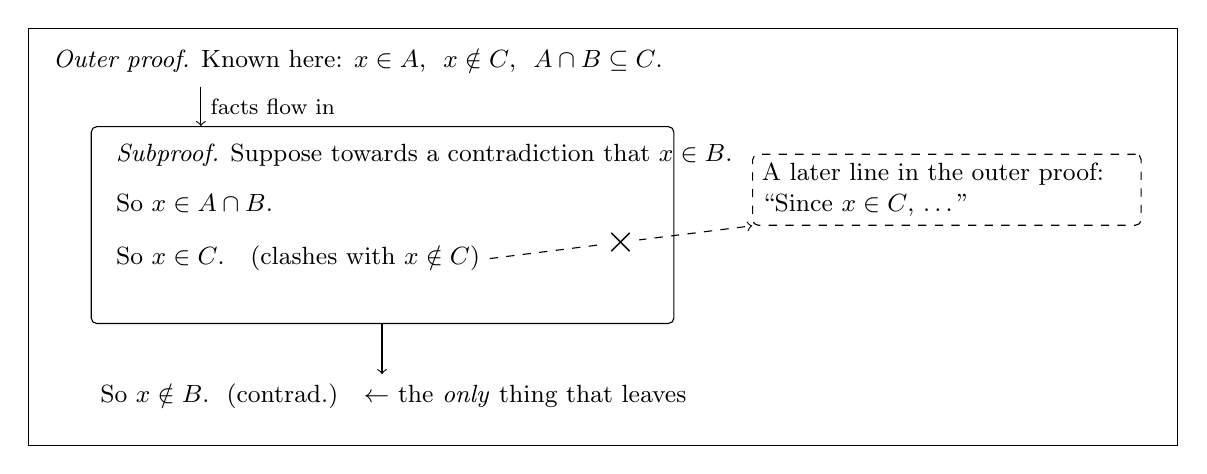
\begin{tikzpicture}[font=\small]
  \node[draw,rectangle,minimum width=14.6cm,minimum height=5.3cm,anchor=north west] (outer) at (0,0) {};
  \node[anchor=north west,align=left] at (0.2,-0.15) {\textit{Outer proof.} Known here: $x\in A$,\ \ $x\notin C$,\ \ $A\cap B\subseteq C$.};
  \draw[->] (2.2,-0.75) -- (2.2,-1.25) node[midway,right,font=\footnotesize] {facts flow in};
  \node[draw,rounded corners=2pt,minimum width=7.4cm,minimum height=2.5cm,anchor=north west] (inner) at (0.8,-1.25) {};
  \node[anchor=north west,align=left] (i1) at (1.0,-1.35) {\textit{Subproof.} Suppose towards a contradiction that $x\in B$.};
  \node[anchor=north west,align=left] (i2) at (1.0,-2.0) {So $x\in A\cap B$.};
  \node[anchor=north west,align=left] (i3) at (1.0,-2.65) {So $x\in C$.\quad (clashes with $x\notin C$)};
  \draw[->] (4.5,-3.75) -- (4.5,-4.4);
  \node[anchor=north west,align=left] (out) at (0.8,-4.4) {So $x\notin B$.\ \ (contrad.)\quad $\leftarrow$ the \emph{only} thing that leaves};
  \node[draw,dashed,rounded corners=2pt,align=left,text width=4.7cm,anchor=north west] (later) at (9.2,-1.6)
     {A later line in the outer proof: ``Since $x\in C$, \dots''};
  \draw[->,dashed] (i3.east) -- node[pos=0.5,fill=white,inner sep=1pt,font=\Large] {$\times$} (later.south west);
\end{tikzpicture}
\end{center}

The dashed arrow is the mistake. $x\in C$ was only true \emph{if} $x\in B$, and the whole point of the subproof was to show that $x\in B$ is false. Citing $x\in C$ outside would be citing something you now know rests on a false assumption. Same story with cases: what you prove inside Case 1 was only true in Case 1. Proof by Cases lets you export one thing, the common conclusion $Z$ you reached in \emph{both} cases.

\subsection{Choosing your move}

Most of being good at these is reading two things: the shape of your goal, and the shape of what you hold. Start from the goal, because it decides the frame of the whole proof.

\begin{figure}[H]
\centering
\begin{tikzpicture}
  \node[softbox,text width=6.2cm,anchor=north west] (start) at (-2.9,0) {Look at your \textbf{goal}. What shape is it?};
  \matrix[matrix of nodes,anchor=north west,column sep=0.75cm,row sep=0.16cm,
    nodes={draw,rectangle,align=left,font=\small,inner sep=3pt},
    column 1/.style={nodes={text width=4.1cm}},
    column 2/.style={nodes={text width=9.1cm}}] (g) at (-2.0,-0.8) {
    ``every \dots'', ``for any \dots'' & univ.\ intro.: name a fresh, arbitrary object with the premise property; write the Goal.\\
    ``if $P$, then $Q$'' & impl.\ intro.: assume $P$, make $Q$ the goal. With ``for any'', fold both into one opening line.\\
    $X\subseteq Y$ & It's universal (def.\ of $\subseteq$). Let $x\in X$, subgoal $x\in Y$; close with (univ.\ intro., def.\ of $\subseteq$).\\
    $X=Y$ & Two $\subseteq$ subproofs: $X\subseteq Y$, then $Y\subseteq X$.\\
    $x\in A\cap B$ & Get $x\in A$ and $x\in B$ separately, then (def.\ of $\cap$).\\
    $x\in A\cup B$ & Get \emph{one} side, then (weak.) and (def.\ of $\cup$). Aim at the side you can reach.\\
    $x\in A-B$ & Get $x\in A$ and $x\notin B$, then (def.\ of $-$).\\
    $x\in\overline{A}$ & Get $x\notin A$, then (def.\ of compl.).\\
    $x\notin S$, or ``not $P$'' & contrad.: ``Suppose towards a contradiction that $x\in S$'', then hunt for a fact and its opposite.\\
    You suspect it's false & Counterexample: specific sets that make the premise true and the conclusion false.\\
  };
  \draw (-2.4,0 |- start.south) -- (-2.4,0 |- g-10-1.west);
  \foreach \i in {1,...,10} { \draw[->] (-2.4,0 |- g-\i-1.west) -- (g-\i-1.west); \draw[->] (g-\i-1.east) -- (g-\i-2.west); }
\end{tikzpicture}
\caption{Goal shape $\to$ first move. Work top-down: the outer shape first (``for any \dots, if \dots, then $X\subseteq Y$''), then the shape of each subgoal as it appears.}
\label{fig:goalchooser}
\end{figure}

Once the frame is up, you're inside a subproof holding some facts. Now the question flips: what can I \emph{do} with what I have?

\begin{figure}[H]
\centering
\begin{tikzpicture}[
  hold/.style={draw,rectangle,align=left,font=\small,text width=3.3cm,inner sep=3pt},
  move/.style={draw,rectangle,align=left,font=\small,text width=6.6cm,inner sep=3pt},
  ask/.style={draw,diamond,aspect=2.3,align=center,font=\footnotesize,inner sep=1pt,text width=2.3cm},
  yn/.style={font=\footnotesize,fill=white,inner sep=1pt}]
  \node[font=\small\itshape] at (1.8,0.55) {You hold \dots};
  \node[font=\small\itshape] at (12.4,0.55) {Your move};
  \node[hold] (h1) at (1.8,0) {$x\in A\cap B$};
  \node[move] (m1) at (12.4,0) {Split it: $x\in A$, and $x\in B$. (def.\ of $\cap$)};
  \node[hold] (h2) at (1.8,-0.85) {$x\in A-B$};
  \node[move] (m2) at (12.4,-0.85) {Split it: $x\in A$, and $x\notin B$. (def.\ of $-$)};
  \node[hold] (h3) at (1.8,-1.7) {$x\in\overline{A}$};
  \node[move] (m3) at (12.4,-1.7) {$x\notin A$. (def.\ of compl.)};
  \foreach \i in {1,2,3} \draw[->] (h\i) -- (m\i);
  % or
  \node[hold] (h4) at (1.8,-3.35) {$x\in A\cup B$, so ``$x\in A$ or $x\in B$'' (def.\ of $\cup$)};
  \node[ask] (q4) at (6.4,-3.35) {Is one side already known false?};
  \node[move] (y4) at (12.4,-2.75) {disj.\ syll.: conclude the other side.};
  \node[move] (n4) at (12.4,-3.95) {pf.\ by cases: one subproof per side; reach the same $Z$ in both.};
  \draw[->] (h4) -- (q4);
  \draw[->] (q4.north) |- node[yn,pos=0.75] {yes} (y4.west);
  \draw[->] (q4.south) |- node[yn,pos=0.75] {no} (n4.west);
  % subset
  \node[hold] (h5) at (1.8,-6.0) {A subset fact $A\subseteq B$};
  \node[ask] (q5) at (6.4,-6.0) {Do you have a \emph{member} of $A$?};
  \node[move] (y5) at (12.4,-5.4) {appl.: that member is in $B$. (appl., def.\ of $\subseteq$)};
  \node[move] (n5) at (12.4,-6.6) {You only have $x\notin A$? Then \textbf{nothing} follows about $B$. Look for another route.};
  \draw[->] (h5) -- (q5);
  \draw[->] (q5.north) |- node[yn,pos=0.75] {yes} (y5.west);
  \draw[->] (q5.south) |- node[yn,pos=0.75] {no} (n5.west);
  % contradiction
  \node[hold] (h6) at (1.8,-8.15) {Some $Y$ and also not-$Y$, inside a subproof that assumed $X$};
  \node[move] (m6) at (12.4,-8.15) {Close it: $X$ is false. Name $X$ and both clashing facts. (contrad.)};
  \draw[->] (h6) -- (m6);
  \node[hold] (h7) at (1.8,-9.45) {A fact from inside a closed subproof};
  \node[move] (m7) at (12.4,-9.45) {Unusable. Only the closing line's conclusion survives.};
  \draw[->] (h7) -- (m7);
\end{tikzpicture}
\caption{What you hold $\to$ next move. The two diamonds are where most wrong steps come from: using disj.\ syll.\ without a side ruled out, and using a subset fact without a member.}
\label{fig:holdchooser}
\end{figure}

\subsubsection{The classic invalid step}

This one deserves its own heading because it's the single most common way to wreck a proof. You hold $x\notin A$ and $A\subseteq B$, and you write ``so $x\notin B$ (appl.)''.

It's invalid. $A\subseteq B$ talks about members of $A$: every one of them is in $B$. It says nothing at all about things outside $A$. Picture $A$ as a small circle inside a big circle $B$. A point outside the small circle can easily sit inside the big one. Application needs an object \emph{with} the property; $x\notin A$ is the object \emph{without} it.

If you genuinely need $x\notin B$, the route is a contradiction subproof: suppose $x\in B$, and find something that breaks. Whether that works depends on what else you know. Sometimes it doesn't work because the claim is false.

\subsection{Worked proofs}

Each proof below starts with the plan, the way you'd think it through on scratch paper, and then the finished proof. Read the plan; it's the part that transfers to new problems.

\subsubsection{A plain subset proof: unpack, apply, pack up}

\textbf{Claim.} For any sets $A$, $B$, $C$ in a universe $\mathcal{U}$, if $A\subseteq B-C$, then $A\subseteq B\cap\overline{C}$.

\emph{Plan.} Goal shape is $A\subseteq\dots$, so: let $x\in A$, subgoal $x\in B\cap\overline{C}$. That's an $\cap$, so I need $x\in B$ and $x\in\overline{C}$ separately, and $x\in\overline{C}$ means $x\notin C$. What do I hold? A member of $A$ and the fact $A\subseteq B-C$. That's exactly the setup for appl.

\begin{center}
\begin{tikzpicture}
  \prfstart
  \prfline{a1}{p0}{1}{1}{Let $A,B,C$ be sets in $\mathcal{U}$ and assume $A\subseteq B-C$.}{(Goal: $A\subseteq B\cap\overline{C}$)}
  \prfline{a2}{a1}{2}{2}{Let $x\in A$.}{(Subgoal: $x\in B\cap\overline{C}$)}
  \prfline{a3}{a2}{2}{3}{Since $x\in A$ and $A\subseteq B-C$, $x\in B-C$.}{(appl., def.\ of $\subseteq$)}
  \prfline{a4}{a3}{2}{4}{So $x\in B$ and $x\notin C$.}{(def.\ of $-$)}
  \prfline{a5}{a4}{2}{5}{Since $x\notin C$, $x\in\overline{C}$.}{(def.\ of compl.)}
  \prfline{a6}{a5}{2}{6}{We have $x\in B$ (line 4) and $x\in\overline{C}$, so $x\in B\cap\overline{C}$.}{(def.\ of $\cap$)}
  \prfline{a7}{a6}{1}{7}{We chose an arbitrary $x\in A$ and proved $x\in B\cap\overline{C}$, so $A\subseteq B\cap\overline{C}$.}{(univ.\ intro., def.\ of $\subseteq$)}
  \prfline{a8}{a7}{0}{8}{We chose sets $A,B,C$ with $A\subseteq B-C$ and proved $A\subseteq B\cap\overline{C}$, which proves the claim.\prfqed}{(univ.\ intro.)}
  \prfscope{a1}{a7}{1}{3.6cm}
  \prfscope{a2}{a6}{2}{1.2cm}
\end{tikzpicture}
\end{center}

Notice the rhythm: definitions to unpack (line 4), one rule to move information (line 3), definitions to pack up (lines 5 and 6). Line 3 uses appl.\ and def.\ of $\subseteq$ together; that's one rule plus one definition, so it's allowed.

\subsubsection{Weakening into a union}

\textbf{Claim.} For any sets $A$, $B$, $C$, if $B\subseteq C$, then $A\cap B\subseteq (C-A)\cup(A\cap C)$.

\emph{Plan.} Let $x\in A\cap B$; subgoal $x\in (C-A)\cup(A\cap C)$. The goal is a union, so I only need one side. Which one? $x\in A$, so $x\in C-A$ is hopeless (it would need $x\notin A$). Aim for $A\cap C$: I have $x\in A$, and I can get $x\in C$ by feeding $x\in B$ into $B\subseteq C$.

\begin{center}
\begin{tikzpicture}
  \prfstart
  \prfline{b1}{p0}{1}{1}{Let $A,B,C$ be sets and assume $B\subseteq C$.}{(Goal: $A\cap B\subseteq (C-A)\cup(A\cap C)$)}
  \prfline{b2}{b1}{2}{2}{Let $x\in A\cap B$.}{(Subgoal: $x\in (C-A)\cup(A\cap C)$)}
  \prfline{b3}{b2}{2}{3}{So $x\in A$ and $x\in B$.}{(def.\ of $\cap$)}
  \prfline{b4}{b3}{2}{4}{Since $x\in B$ and $B\subseteq C$, $x\in C$.}{(appl., def.\ of $\subseteq$)}
  \prfline{b5}{b4}{2}{5}{We have $x\in A$ and $x\in C$, so $x\in A\cap C$.}{(def.\ of $\cap$)}
  \prfline{b6}{b5}{2}{6}{So $x\in C-A$ or $x\in A\cap C$.}{(weak.)}
  \prfline{b7}{b6}{2}{7}{So $x\in (C-A)\cup(A\cap C)$.}{(def.\ of $\cup$)}
  \prfline{b8}{b7}{1}{8}{We chose an arbitrary $x\in A\cap B$ and proved $x\in (C-A)\cup(A\cap C)$, so $A\cap B\subseteq (C-A)\cup(A\cap C)$.}{(univ.\ intro., def.\ of $\subseteq$)}
  \prfline{b9}{b8}{0}{9}{We chose sets $A,B,C$ with $B\subseteq C$ and proved $A\cap B\subseteq (C-A)\cup(A\cap C)$, which proves the claim.\prfqed}{(univ.\ intro.)}
  \prfscope{b1}{b8}{1}{3.2cm}
  \prfscope{b2}{b7}{2}{1.6cm}
\end{tikzpicture}
\end{center}

Line 6 is the whole point. Weakening lets you tack on \emph{any} statement with ``or'', even one you know is false, and on either side. Lines 6 and 7 could be merged into ``So $x\in(C-A)\cup(A\cap C)$ (weak., def.\ of $\cup$)'', since that's one rule plus one definition. Both versions are fine.

The trap here is starting with the wrong side. If you'd aimed at $x\in C-A$ you'd have stalled, and the temptation is to fudge. Before committing to a side, ask whether that side can even be true for your $x$.

\subsubsection{Disjunctive syllogism: kill one option}

\textbf{Claim.} For any sets $A$, $B$, $C$, if $B\subseteq A\cup C$, then $B-A\subseteq C\cap B$.

\emph{Plan.} Let $x\in B-A$, so $x\in B$ and $x\notin A$. Subgoal $x\in C\cap B$; I already have $x\in B$, so I really need $x\in C$. Feeding $x\in B$ into the hypothesis gives $x\in A\cup C$, an ``or''. One side ($x\in A$) is already known false. That's disj.\ syll.

\begin{center}
\begin{tikzpicture}
  \prfstart
  \prfline{c1}{p0}{1}{1}{Let $A,B,C$ be sets and assume $B\subseteq A\cup C$.}{(Goal: $B-A\subseteq C\cap B$)}
  \prfline{c2}{c1}{2}{2}{Let $x\in B-A$.}{(Subgoal: $x\in C\cap B$)}
  \prfline{c3}{c2}{2}{3}{So $x\in B$ and $x\notin A$.}{(def.\ of $-$)}
  \prfline{c4}{c3}{2}{4}{Since $x\in B$ and $B\subseteq A\cup C$, $x\in A\cup C$.}{(appl., def.\ of $\subseteq$)}
  \prfline{c5}{c4}{2}{5}{So $x\in A$ or $x\in C$.}{(def.\ of $\cup$)}
  \prfline{c6}{c5}{2}{6}{Since $x\in A$ or $x\in C$, and $x\notin A$ (line 3), $x\in C$.}{(disj.\ syll.)}
  \prfline{c7}{c6}{2}{7}{We have $x\in C$ and $x\in B$ (line 3), so $x\in C\cap B$.}{(def.\ of $\cap$)}
  \prfline{c8}{c7}{1}{8}{We chose an arbitrary $x\in B-A$ and proved $x\in C\cap B$, so $B-A\subseteq C\cap B$.}{(univ.\ intro., def.\ of $\subseteq$)}
  \prfline{c9}{c8}{0}{9}{We chose sets $A,B,C$ with $B\subseteq A\cup C$ and proved $B-A\subseteq C\cap B$, which proves the claim.\prfqed}{(univ.\ intro.)}
  \prfscope{c1}{c8}{1}{3.4cm}
  \prfscope{c2}{c7}{2}{1.2cm}
\end{tikzpicture}
\end{center}

Lines 4 and 5 can't be merged: that would be appl.\ plus \emph{two} definitions ($\subseteq$ and $\cup$). Disj.\ syll.\ needs the \emph{negation} of one side. Knowing that one side is \emph{true} gives you nothing about the other, because inclusive ``or'' allows both. That mistake shows up again in the proof-checking section.

\subsubsection{Proof by cases: when you can't rule either side out}

\textbf{Claim.} For any sets $A$, $B$, $C$, if $A\subseteq B\cup C$ and $A\cap B\subseteq C$, then $A\subseteq C$.

\emph{Plan.} Let $x\in A$; subgoal $x\in C$. Apply the first hypothesis: $x\in B$ or $x\in C$. Is either side known false? No. So split. If $x\in C$, I'm done on the spot. If $x\in B$, then together with $x\in A$ (which I still have, because it came from the outer proof) I get $x\in A\cap B$, and the second hypothesis finishes it.

\begin{center}
\begin{tikzpicture}
  \prfstart
  \prfline{d1}{p0}{1}{1}{Let $A,B,C$ be sets and assume $A\subseteq B\cup C$ and $A\cap B\subseteq C$.}{(Goal: $A\subseteq C$)}
  \prfline{d2}{d1}{2}{2}{Let $x\in A$.}{(Subgoal: $x\in C$)}
  \prfline{d3}{d2}{2}{3}{Since $x\in A$ and $A\subseteq B\cup C$, $x\in B\cup C$.}{(appl., def.\ of $\subseteq$)}
  \prfline{d4}{d3}{2}{4}{So $x\in B$ or $x\in C$.}{(def.\ of $\cup$)}
  \prfline{d5}{d4}{3}{5}{Case 1: assume $x\in B$.}{(Case goal: $x\in C$)}
  \prfline{d6}{d5}{3}{6}{We have $x\in A$ (line 2) and $x\in B$, so $x\in A\cap B$.}{(def.\ of $\cap$)}
  \prfline{d7}{d6}{3}{7}{Since $x\in A\cap B$ and $A\cap B\subseteq C$, $x\in C$.}{(appl., def.\ of $\subseteq$)}
  \prfline{d8}{d7}{3}{8}{Case 2: assume $x\in C$. This is already the case goal.}{(Case goal: $x\in C$)}
  \prfline{d9}{d8}{2}{9}{We know $x\in B$ or $x\in C$ (line 4), and both cases (lines 5--7 and line 8) give $x\in C$, so $x\in C$.}{(pf.\ by cases)}
  \prfline{d10}{d9}{1}{10}{We chose an arbitrary $x\in A$ and proved $x\in C$, so $A\subseteq C$.}{(univ.\ intro., def.\ of $\subseteq$)}
  \prfline{d11}{d10}{0}{11}{We chose sets $A,B,C$ with $A\subseteq B\cup C$ and $A\cap B\subseteq C$ and proved $A\subseteq C$, which proves the claim.\prfqed}{(univ.\ intro.)}
  \prfscope{d1}{d10}{1}{5.6cm}
  \prfscope{d2}{d9}{2}{1.0cm}
  \prfscope{d5}{d7}{3}{2.6cm}
  \prfscope{d8}{d8}{3}{2.6cm}
\end{tikzpicture}
\end{center}

Two things to notice. Line 6 reaches \emph{out} of Case 1 to grab $x\in A$ from line 2. That's legal: facts flow into a subproof. And line 7's $x\in C$ isn't usable after Case 1 closes; line 9 is what carries $x\in C$ out, and only because \emph{both} cases reached it. A case that's trivially done (Case 2 here) still has to appear, so the reader sees you covered it.

\subsubsection{Proof by contradiction: proving a ``not''}

\textbf{Claim.} For any sets $A$, $B$, $C$ in a universe $\mathcal{U}$, if $A\cap B\subseteq C$, then $A-C\subseteq\overline{B}$.

\begin{center}
\begin{minipage}[c]{0.56\linewidth}
\emph{Plan.} Let $x\in A-C$, so $x\in A$ and $x\notin C$. Subgoal $x\in\overline{B}$, which means $x\notin B$. That's a ``not'' goal, and nothing I hold says anything about $B$ directly. So: assume the bad thing, $x\in B$, and watch it break. With $x\in A$ and $x\in B$ I get $x\in A\cap B$, then $x\in C$ from the hypothesis, and that clashes with $x\notin C$.\par\smallskip
\emph{Sanity check (right).} $A-C$ is the grey part plus the cross-hatched part. The cross-hatched part ($A\cap B$ outside $C$) is empty by the hypothesis, so all that's left of $A-C$ is grey, and grey misses $B$ entirely. A picture isn't a proof, but it tells you the claim is worth trying to prove.
\end{minipage}\hfill
\begin{minipage}[c]{0.4\linewidth}
\centering
\begin{tikzpicture}[scale=0.95]
  \def\cA{(0,0) circle (1.05)}
  \def\cB{(1.25,0) circle (1.05)}
  \def\cC{(0.62,-1.05) circle (1.05)}
  \begin{scope}\clip \cA; \fill[gray!35] \cA; \end{scope}
  \begin{scope}\clip \cA; \clip \cB; \fill[white] \cB; \fill[pattern=crosshatch] \cB; \end{scope}
  \begin{scope}\clip \cA; \fill[white] \cC; \end{scope}
  \draw \cA; \draw \cB; \draw \cC;
  \draw (-1.4,-2.45) rectangle (2.65,1.3);
  \node[font=\scriptsize,anchor=north west] at (-1.4,1.3) {$\mathcal{U}$};
  \node[font=\small] at (-0.55,0.45) {$A$};
  \node[font=\small] at (1.8,0.45) {$B$};
  \node[font=\small] at (0.62,-1.75) {$C$};
  \node[font=\scriptsize,align=center,fill=white,inner sep=1pt] at (0.62,1.6) {hatched: $A\cap B$ outside $C$ (empty)};
\end{tikzpicture}
\end{minipage}
\end{center}

\begin{center}
\begin{tikzpicture}
  \prfstart
  \prfline{e1}{p0}{1}{1}{Let $A,B,C$ be sets in $\mathcal{U}$ and assume $A\cap B\subseteq C$.}{(Goal: $A-C\subseteq\overline{B}$)}
  \prfline{e2}{e1}{2}{2}{Let $x\in A-C$.}{(Subgoal: $x\in\overline{B}$)}
  \prfline{e3}{e2}{2}{3}{So $x\in A$ and $x\notin C$.}{(def.\ of $-$)}
  \prfline{e4}{e3}{3}{4}{Suppose towards a contradiction that $x\in B$.}{(Goal: a contradiction)}
  \prfline{e5}{e4}{3}{5}{We have $x\in A$ (line 3) and $x\in B$, so $x\in A\cap B$.}{(def.\ of $\cap$)}
  \prfline{e6}{e5}{3}{6}{Since $x\in A\cap B$ and $A\cap B\subseteq C$, $x\in C$.}{(appl., def.\ of $\subseteq$)}
  \prfline{e7}{e6}{2}{7}{I assumed $x\in B$ and proved $x\in C$, but $x\notin C$ (line 3). So $x\notin B$.}{(contrad.)}
  \prfline{e8}{e7}{2}{8}{So $x\in\overline{B}$.}{(def.\ of compl.)}
  \prfline{e9}{e8}{1}{9}{We chose an arbitrary $x\in A-C$ and proved $x\in\overline{B}$, so $A-C\subseteq\overline{B}$.}{(univ.\ intro., def.\ of $\subseteq$)}
  \prfline{e10}{e9}{0}{10}{We chose sets $A,B,C$ with $A\cap B\subseteq C$ and proved $A-C\subseteq\overline{B}$, which proves the claim.\prfqed}{(univ.\ intro.)}
  \prfscope{e1}{e9}{1}{4.6cm}
  \prfscope{e2}{e8}{2}{1.2cm}
  \prfscope{e4}{e6}{3}{5.4cm}
\end{tikzpicture}
\end{center}

Line 7 is the closing line, and it does three jobs: names the assumption ($x\in B$), names both clashing facts ($x\in C$ from inside, $x\notin C$ from outside), and states what follows ($x\notin B$). Leave out any of those and you'll lose points even if the logic is right.

A few more things about contradiction:

\begin{itemize}
  \item It's the tool for any $\notin$ goal, and for $x\in\overline{A}$ and $x\in A-B$, since those both hide a $\notin$.
  \item It also works for positive goals. Assume $x\notin B$, break it, and you've shown ``$x\notin B$'' is false, which is $x\in B$. Practice problem 7 uses this.
  \item Subproofs nest. You can open a contradiction inside a contradiction (Practice problem 13). Keep the bars straight and close the inner one first.
  \item The clash can be any statement and its opposite. Usually one half comes from inside the subproof and the other half from outside.
\end{itemize}

\subsubsection{Set equality: two subset proofs}

To prove $X=Y$, prove $X\subseteq Y$ and $Y\subseteq X$, then put them together. The notes give this as the way to show two sets are equal (\S2.5.1), but ``def.\ of $=$'' isn't in the notes' table of definitions for constrained proofs. Check the rule sheet on your test. If it lists set equality, cite it as below. If it doesn't, you can still do both directions, but ask how they want the last line justified.

\textbf{Claim.} For any sets $A$, $B$ in a universe $\mathcal{U}$, $A-B=A\cap\overline{B}$.

\begin{center}
\begin{tikzpicture}
  \prfstart
  \prfline{q1}{p0}{1}{1}{Let $A,B$ be sets in $\mathcal{U}$.}{(Goal: $A-B=A\cap\overline{B}$)}
  \prfline{q2}{q1}{2}{2}{Let $x\in A-B$.}{(Subgoal: $x\in A\cap\overline{B}$)}
  \prfline{q3}{q2}{2}{3}{So $x\in A$ and $x\notin B$.}{(def.\ of $-$)}
  \prfline{q4}{q3}{2}{4}{Since $x\notin B$, $x\in\overline{B}$.}{(def.\ of compl.)}
  \prfline{q5}{q4}{2}{5}{We have $x\in A$ and $x\in\overline{B}$, so $x\in A\cap\overline{B}$.}{(def.\ of $\cap$)}
  \prfline{q6}{q5}{1}{6}{We chose an arbitrary $x\in A-B$ and proved $x\in A\cap\overline{B}$, so $A-B\subseteq A\cap\overline{B}$.}{(univ.\ intro., def.\ of $\subseteq$)}
  \prfline{q7}{q6}{2}{7}{Let $y\in A\cap\overline{B}$.}{(Subgoal: $y\in A-B$)}
  \prfline{q8}{q7}{2}{8}{So $y\in A$ and $y\in\overline{B}$.}{(def.\ of $\cap$)}
  \prfline{q9}{q8}{2}{9}{Since $y\in\overline{B}$, $y\notin B$.}{(def.\ of compl.)}
  \prfline{q10}{q9}{2}{10}{We have $y\in A$ and $y\notin B$, so $y\in A-B$.}{(def.\ of $-$)}
  \prfline{q11}{q10}{1}{11}{We chose an arbitrary $y\in A\cap\overline{B}$ and proved $y\in A-B$, so $A\cap\overline{B}\subseteq A-B$.}{(univ.\ intro., def.\ of $\subseteq$)}
  \prfline{q12}{q11}{1}{12}{By lines 6 and 11, $A-B\subseteq A\cap\overline{B}$ and $A\cap\overline{B}\subseteq A-B$, so $A-B=A\cap\overline{B}$.}{(def.\ of $=$, if your sheet lists it)}
  \prfline{q13}{q12}{0}{13}{We chose arbitrary sets $A,B$ and proved $A-B=A\cap\overline{B}$, which proves the claim.\prfqed}{(univ.\ intro.)}
  \prfscope{q1}{q12}{1}{2.4cm}
  \prfscope{q2}{q5}{2}{1.2cm}
  \prfscope{q7}{q10}{2}{1.4cm}
\end{tikzpicture}
\end{center}

The second direction uses $y$ instead of $x$. Reusing $x$ would actually be legal, since the first $x$ died when its subproof closed at line 5, but a new letter keeps the reader from wondering.

One more thing worth knowing. The rule list has no ``either $x\in B$ or $x\notin B$''. So if your plan is ``split on whether $x$ is in $B$'', you can't just write that line. You'd need it handed to you as a given ``or'' (to use cases) or you'd restructure the argument around a contradiction instead.

\subsection{Disproving a claim: counterexamples}

A universal claim is false as soon as one example breaks it. You don't write a constrained proof for this (the notes say so), just specific sets plus the reason they work.

\textbf{Claim.} For any sets $A$, $B$, $C$, if $A\cap C\subseteq B\cap C$, then $A\subseteq B$. True or false?

This looks like ``cancel the $\cap C$ from both sides'', which is exactly why it's suspicious. Try to prove it and you get stuck fast: from $x\in A$ you can't reach anything, because the hypothesis only talks about members of $A\cap C$, and you don't know $x\in C$.

\textbf{How to hunt.} Force the premise true and the conclusion false, then solve for the sets.
\begin{enumerate}
  \item For the conclusion to fail, some element must be in $A$ but not in $B$. Call it $1$: $1\in A$, $1\notin B$.
  \item Now protect the premise. If $1$ were in $C$, then $1\in A\cap C$ would have to be in $B\cap C$, so in $B$. It isn't. So keep $1$ out of $C$.
  \item Use the smallest sets that do the job: $A=\{1\}$, $B=\varnothing$, $C=\varnothing$.
\end{enumerate}

\textbf{Write-up.} Let $A=\{1\}$, $B=\varnothing$, $C=\varnothing$. Then $A\cap C=\varnothing$ and $B\cap C=\varnothing$, so $A\cap C\subseteq B\cap C$. But $1\in A$ and $1\notin B$, so $A\not\subseteq B$. The premise holds and the conclusion fails, so the claim is false.

Always name the specific element that breaks the conclusion ($1$ here). ``Clearly $A\not\subseteq B$'' is weaker than pointing at the element.

\subsection{Checking a proof someone else wrote}

The notes warn that a test may hand you a proof attempt and ask whether it's valid: for each line, name the rule it uses, or say it's invalid. For every line, ask three questions.

\begin{enumerate}
  \item \emph{Do the facts it cites exist, and are they in scope?} They must appear on an earlier line, and not inside a subproof that has already closed.
  \item \emph{Does the rule fit the facts, in the right direction?} Appl.\ needs a \emph{member} of the left-hand set. Disj.\ syll.\ needs one side shown \emph{false}. Contrad.\ needs a statement and its opposite. Weakening only builds ``or'', it never removes one.
  \item \emph{Is it one rule plus at most one definition?} And are both on the list?
\end{enumerate}

\textbf{Walkthrough.} Claim: for any sets $A$, $B$, $C$, if $A\subseteq B\cup C$, then $A\cap C\subseteq B$. Here's an attempt, with the attempt's own labels.

\begin{center}
\begin{tikzpicture}
  \prfstart
  \prfline{w1}{p0}{1}{1}{Let $A,B,C$ be sets and assume $A\subseteq B\cup C$.}{(Goal: $A\cap C\subseteq B$)}
  \prfline{w2}{w1}{2}{2}{Let $x\in A\cap C$.}{(Subgoal: $x\in B$)}
  \prfline{w3}{w2}{2}{3}{So $x\in A$ and $x\in C$.}{(def.\ of $\cap$)}
  \prfline{w4}{w3}{2}{4}{Since $x\in A$ and $A\subseteq B\cup C$, $x\in B\cup C$.}{(appl., def.\ of $\subseteq$)}
  \prfline{w5}{w4}{2}{5}{So $x\in B$ or $x\in C$.}{(def.\ of $\cup$)}
  \prfline{w6}{w5}{2}{6}{Since $x\in B$ or $x\in C$, and $x\in C$ (line 3), $x\in B$.}{(disj.\ syll.)\quad \textbf{invalid}}
  \prfline{w7}{w6}{1}{7}{We chose an arbitrary $x\in A\cap C$ and proved $x\in B$, so $A\cap C\subseteq B$.}{(univ.\ intro., def.\ of $\subseteq$)}
  \prfline{w8}{w7}{0}{8}{We chose sets $A,B,C$ with $A\subseteq B\cup C$ and proved $A\cap C\subseteq B$, which proves the claim.\prfqed}{(univ.\ intro.)}
  \prfscope{w1}{w7}{1}{3.4cm}
  \prfscope{w2}{w6}{2}{1.2cm}
\end{tikzpicture}
\end{center}

Lines 1--5 pass all three questions. Line 6 fails question 2. Disj.\ syll.\ needs one side to be \emph{false}; here one side ($x\in C$) is known \emph{true}. With inclusive ``or'', knowing one side is true tells you nothing about the other. Lines 7 and 8 are correctly formed but rest on line 6, so the proof is broken.

Is the claim itself false, or is the proof just bad? Hunt: I want $x\in A\cap C$ with $x\notin B$, and the premise only needs $x\in B\cup C$, which $x\in C$ already gives. So $A=\{1\}$, $B=\varnothing$, $C=\{1\}$: then $A\subseteq B\cup C=\{1\}$, but $1\in A\cap C$ and $1\notin B$. The claim is false, which is why no valid proof could finish.

When you grade a line, grade the line, not the claim. A step can be invalid even when the claim is true, and a proof of a false claim always has at least one invalid step somewhere.

\subsection{When you're stuck}

Getting stuck is normal, and the notes go further: being able to get stuck is the most important proof-writing skill. Someone who never gets stuck will ``prove'' false claims. When you stall, there are three possible reasons, and you can't tell which right away:

\begin{enumerate}
  \item \emph{You haven't found the right strategy yet.} Re-read the goal's shape (Figure~\ref{fig:goalchooser}). Are you holding an ``or'' you haven't split? A $\notin$ goal you're trying to reach directly instead of by contradiction?
  \item \emph{You made an error earlier, or copied the claim wrong.} Run the three questions over each line you've written. Compare the claim on your page to the one on the test, symbol by symbol. $A-B$ and $B-A$ are different sets.
  \item \emph{The claim is false.} Hunt for a counterexample: force the premise true and the conclusion false, then build the smallest sets that do it. If you find one, you're done. On a true/false item, that counterexample is the answer.
\end{enumerate}

\begin{notebox}
\textbf{Partial credit, straight from the notes:} an incomplete proof with no errors earns more than a ``complete'' proof with a logical error in it. If you can't finish, write the frame correctly (opening lines, goals, the closing lines you'd use), fill in every step you can justify, and leave a visible gap with a note like ``still need $x\in C$''. Never write ``so $x\in C$'' with a rule you know doesn't fit. A confident wrong step costs you more than an honest gap.
\end{notebox}

\subsection{Practice}

All claims are about arbitrary sets in a universe $\mathcal{U}$ (needed wherever a complement appears). Write constrained proofs using only the five definitions and the rules in this chapter.

\textbf{Write a proof.}
\begin{enumerate}[label=\arabic*.,leftmargin=1.8em]
  \item If $A\subseteq B$, then $A\cap\overline{C}\subseteq B-C$.
  \item If $A\subseteq B$, then $A-C\subseteq (B-C)\cup(C-B)$.
  \item If $A\subseteq B\cup C$ and $A\subseteq\overline{B}$, then $A\subseteq C$.
  \item If $A\subseteq B$ and $C\subseteq B$, then $(A\cap\overline{C})\cup C\subseteq B$.
  \item If $A\subseteq B-C$, then $C\subseteq\overline{A}$.
\end{enumerate}

\textbf{True or false? Decide, then prove it or give a counterexample.}
\begin{enumerate}[label=\arabic*.,leftmargin=1.8em,resume]
  \item If $A\cup C\subseteq B\cup C$, then $A\subseteq B$.
  \item If $A-B\subseteq C$, then $A-C\subseteq B$.
  \item If $A\subseteq B\cup C$, then $A-C\subseteq B-C$.
  \item If $A\cap B\subseteq C$, then $A\cap C\subseteq B$.
\end{enumerate}

\textbf{Check the proof. For each line, name the rule it uses or mark it invalid and say why. Then decide whether the claim is true.}

\begin{enumerate}[label=\arabic*.,leftmargin=1.8em,resume]
  \item Claim: if $B\subseteq C$, then $A-B\subseteq A-C$.
\end{enumerate}

\begin{center}
\begin{tikzpicture}
  \prfstart
  \prfline{x1}{p0}{1}{1}{Let $A,B,C$ be sets and assume $B\subseteq C$.}{(Goal: $A-B\subseteq A-C$)}
  \prfline{x2}{x1}{2}{2}{Let $x\in A-B$.}{(Subgoal: $x\in A-C$)}
  \prfline{x3}{x2}{2}{3}{So $x\in A$ and $x\notin B$.}{(\underline{\hspace{2.2cm}})}
  \prfline{x4}{x3}{2}{4}{Since $x\notin B$ and $B\subseteq C$, $x\notin C$.}{(\underline{\hspace{2.2cm}})}
  \prfline{x5}{x4}{2}{5}{We have $x\in A$ and $x\notin C$, so $x\in A-C$.}{(\underline{\hspace{2.2cm}})}
  \prfline{x6}{x5}{1}{6}{We chose an arbitrary $x\in A-B$ and proved $x\in A-C$, so $A-B\subseteq A-C$.}{(\underline{\hspace{2.2cm}})}
  \prfline{x7}{x6}{0}{7}{We chose sets $A,B,C$ with $B\subseteq C$ and proved $A-B\subseteq A-C$.\prfqed}{(\underline{\hspace{2.2cm}})}
  \prfscope{x1}{x6}{1}{3.4cm}
  \prfscope{x2}{x5}{2}{1.2cm}
\end{tikzpicture}
\end{center}

\begin{enumerate}[label=\arabic*.,leftmargin=1.8em,resume]
  \item Claim: if $A\subseteq B\cup C$ and $C\subseteq A$, then $A\subseteq B$.
\end{enumerate}

\begin{center}
\begin{tikzpicture}
  \prfstart
  \prfline{y1}{p0}{1}{1}{Let $A,B,C$ be sets and assume $A\subseteq B\cup C$ and $C\subseteq A$.}{(Goal: $A\subseteq B$)}
  \prfline{y2}{y1}{2}{2}{Let $x\in A$.}{(Subgoal: $x\in B$)}
  \prfline{y3}{y2}{2}{3}{Since $x\in A$ and $A\subseteq B\cup C$, $x\in B\cup C$.}{(\underline{\hspace{2.2cm}})}
  \prfline{y4}{y3}{2}{4}{So $x\in B$ or $x\in C$.}{(\underline{\hspace{2.2cm}})}
  \prfline{y5}{y4}{3}{5}{Case 1: assume $x\in B$. That's the case goal.}{(Case goal: $x\in B$)}
  \prfline{y6}{y5}{3}{6}{Case 2: assume $x\in C$.}{(Case goal: $x\in B$)}
  \prfline{y7}{y6}{3}{7}{Since $x\in C$ and $C\subseteq A$, $x\in A$.}{(\underline{\hspace{2.2cm}})}
  \prfline{y8}{y7}{3}{8}{From line 5, $x\in B$.}{(\underline{\hspace{2.2cm}})}
  \prfline{y9}{y8}{2}{9}{Both cases give $x\in B$, so $x\in B$.}{(\underline{\hspace{2.2cm}})}
  \prfline{y10}{y9}{1}{10}{We chose an arbitrary $x\in A$ and proved $x\in B$, so $A\subseteq B$.}{(\underline{\hspace{2.2cm}})}
  \prfline{y11}{y10}{0}{11}{We chose sets $A,B,C$ with the two assumptions and proved $A\subseteq B$.\prfqed}{(\underline{\hspace{2.2cm}})}
  \prfscope{y1}{y10}{1}{5.4cm}
  \prfscope{y2}{y9}{2}{1.0cm}
  \prfscope{y5}{y5}{3}{2.6cm}
  \prfscope{y6}{y8}{3}{2.2cm}
\end{tikzpicture}
\end{center}

\textbf{Longer ones.}
\begin{enumerate}[label=\arabic*.,leftmargin=1.8em,resume]
  \item Prove $A\cap(B-C)=(A\cap B)-C$. (Assume your sheet lists def.\ of $=$.)
  \item Prove: if $A-B\subseteq C$ and $B\subseteq C$, then $A\subseteq C$. Hint: you can't split on ``$x\in B$ or $x\notin B$''. Try assuming the conclusion fails.
\end{enumerate}

\subsection{Answers}

Opening and closing lines follow the same pattern every time, so after the first few answers they're written out but not discussed. All true claims were checked by brute force and all counterexamples were tested.

\textbf{1.} Unpack $\cap$ and compl., apply, pack into $-$.

\begin{center}
\begin{tikzpicture}
  \prfstart
  \prfline{r1}{p0}{1}{1}{Let $A,B,C$ be sets in $\mathcal{U}$ and assume $A\subseteq B$.}{(Goal: $A\cap\overline{C}\subseteq B-C$)}
  \prfline{r2}{r1}{2}{2}{Let $x\in A\cap\overline{C}$.}{(Subgoal: $x\in B-C$)}
  \prfline{r3}{r2}{2}{3}{So $x\in A$ and $x\in\overline{C}$.}{(def.\ of $\cap$)}
  \prfline{r4}{r3}{2}{4}{Since $x\in\overline{C}$, $x\notin C$.}{(def.\ of compl.)}
  \prfline{r5}{r4}{2}{5}{Since $x\in A$ and $A\subseteq B$, $x\in B$.}{(appl., def.\ of $\subseteq$)}
  \prfline{r6}{r5}{2}{6}{We have $x\in B$ and $x\notin C$ (line 4), so $x\in B-C$.}{(def.\ of $-$)}
  \prfline{r7}{r6}{1}{7}{We chose an arbitrary $x\in A\cap\overline{C}$ and proved $x\in B-C$, so $A\cap\overline{C}\subseteq B-C$.}{(univ.\ intro., def.\ of $\subseteq$)}
  \prfline{r8}{r7}{0}{8}{We chose sets $A,B,C$ with $A\subseteq B$ and proved $A\cap\overline{C}\subseteq B-C$, which proves the claim.\prfqed}{(univ.\ intro.)}
  \prfscope{r1}{r7}{1}{3.6cm}
  \prfscope{r2}{r6}{2}{1.4cm}
\end{tikzpicture}
\end{center}

\textbf{2.} Get $x\in B-C$, then weaken. Line 6 does the weakening and the def.\ of $\cup$ in one step, which is allowed: one rule plus one definition.

\begin{center}
\begin{tikzpicture}
  \prfstart
  \prfline{r1}{p0}{1}{1}{Let $A,B,C$ be sets and assume $A\subseteq B$.}{(Goal: $A-C\subseteq (B-C)\cup(C-B)$)}
  \prfline{r2}{r1}{2}{2}{Let $x\in A-C$.}{(Subgoal: $x\in (B-C)\cup(C-B)$)}
  \prfline{r3}{r2}{2}{3}{So $x\in A$ and $x\notin C$.}{(def.\ of $-$)}
  \prfline{r4}{r3}{2}{4}{Since $x\in A$ and $A\subseteq B$, $x\in B$.}{(appl., def.\ of $\subseteq$)}
  \prfline{r5}{r4}{2}{5}{We have $x\in B$ and $x\notin C$ (line 3), so $x\in B-C$.}{(def.\ of $-$)}
  \prfline{r6}{r5}{2}{6}{So $x\in (B-C)\cup(C-B)$.}{(weak., def.\ of $\cup$)}
  \prfline{r7}{r6}{1}{7}{We chose an arbitrary $x\in A-C$ and proved $x\in (B-C)\cup(C-B)$, so $A-C\subseteq (B-C)\cup(C-B)$.}{(univ.\ intro., def.\ of $\subseteq$)}
  \prfline{r8}{r7}{0}{8}{We chose sets $A,B,C$ with $A\subseteq B$ and proved $A-C\subseteq (B-C)\cup(C-B)$, which proves the claim.\prfqed}{(univ.\ intro.)}
  \prfscope{r1}{r7}{1}{3.2cm}
  \prfscope{r2}{r6}{2}{1.2cm}
\end{tikzpicture}
\end{center}

\textbf{3.} Apply \emph{both} hypotheses to the same $x$. The second one is what rules out a side for disj.\ syll.

\begin{center}
\begin{tikzpicture}
  \prfstart
  \prfline{r1}{p0}{1}{1}{Let $A,B,C$ be sets in $\mathcal{U}$ and assume $A\subseteq B\cup C$ and $A\subseteq\overline{B}$.}{(Goal: $A\subseteq C$)}
  \prfline{r2}{r1}{2}{2}{Let $x\in A$.}{(Subgoal: $x\in C$)}
  \prfline{r3}{r2}{2}{3}{Since $x\in A$ and $A\subseteq B\cup C$, $x\in B\cup C$.}{(appl., def.\ of $\subseteq$)}
  \prfline{r4}{r3}{2}{4}{So $x\in B$ or $x\in C$.}{(def.\ of $\cup$)}
  \prfline{r5}{r4}{2}{5}{Since $x\in A$ and $A\subseteq\overline{B}$, $x\in\overline{B}$.}{(appl., def.\ of $\subseteq$)}
  \prfline{r6}{r5}{2}{6}{So $x\notin B$.}{(def.\ of compl.)}
  \prfline{r7}{r6}{2}{7}{Since $x\in B$ or $x\in C$ (line 4), and $x\notin B$, $x\in C$.}{(disj.\ syll.)}
  \prfline{r8}{r7}{1}{8}{We chose an arbitrary $x\in A$ and proved $x\in C$, so $A\subseteq C$.}{(univ.\ intro., def.\ of $\subseteq$)}
  \prfline{r9}{r8}{0}{9}{We chose sets $A,B,C$ with $A\subseteq B\cup C$ and $A\subseteq\overline{B}$ and proved $A\subseteq C$, which proves the claim.\prfqed}{(univ.\ intro.)}
  \prfscope{r1}{r8}{1}{5.6cm}
  \prfscope{r2}{r7}{2}{1.0cm}
\end{tikzpicture}
\end{center}

\textbf{4.} The thing you hold is a union with neither side ruled out, so it's cases. Each case uses a different hypothesis.

\begin{center}
\begin{tikzpicture}
  \prfstart
  \prfline{r1}{p0}{1}{1}{Let $A,B,C$ be sets in $\mathcal{U}$ and assume $A\subseteq B$ and $C\subseteq B$.}{(Goal: $(A\cap\overline{C})\cup C\subseteq B$)}
  \prfline{r2}{r1}{2}{2}{Let $x\in (A\cap\overline{C})\cup C$.}{(Subgoal: $x\in B$)}
  \prfline{r3}{r2}{2}{3}{So $x\in A\cap\overline{C}$ or $x\in C$.}{(def.\ of $\cup$)}
  \prfline{r4}{r3}{3}{4}{Case 1: assume $x\in A\cap\overline{C}$.}{(Case goal: $x\in B$)}
  \prfline{r5}{r4}{3}{5}{So $x\in A$ and $x\in\overline{C}$.}{(def.\ of $\cap$)}
  \prfline{r6}{r5}{3}{6}{Since $x\in A$ and $A\subseteq B$, $x\in B$.}{(appl., def.\ of $\subseteq$)}
  \prfline{r7}{r6}{3}{7}{Case 2: assume $x\in C$.}{(Case goal: $x\in B$)}
  \prfline{r8}{r7}{3}{8}{Since $x\in C$ and $C\subseteq B$, $x\in B$.}{(appl., def.\ of $\subseteq$)}
  \prfline{r9}{r8}{2}{9}{We know $x\in A\cap\overline{C}$ or $x\in C$ (line 3), and both cases (lines 4--6, 7--8) give $x\in B$, so $x\in B$.}{(pf.\ by cases)}
  \prfline{r10}{r9}{1}{10}{We chose an arbitrary $x\in (A\cap\overline{C})\cup C$ and proved $x\in B$, so $(A\cap\overline{C})\cup C\subseteq B$.}{(univ.\ intro., def.\ of $\subseteq$)}
  \prfline{r11}{r10}{0}{11}{We chose sets $A,B,C$ with $A\subseteq B$ and $C\subseteq B$ and proved $(A\cap\overline{C})\cup C\subseteq B$, which proves the claim.\prfqed}{(univ.\ intro.)}
  \prfscope{r1}{r10}{1}{5.4cm}
  \prfscope{r2}{r9}{2}{2.2cm}
  \prfscope{r4}{r6}{3}{3.2cm}
  \prfscope{r7}{r8}{3}{2.2cm}
\end{tikzpicture}
\end{center}

The $x\in\overline{C}$ in line 5 is never used. That's fine; unpacking gives you both halves whether you need them or not.

\textbf{5.} The goal $x\in\overline{A}$ means $x\notin A$, so contradiction. The clash comes from the hypothesis handing you $x\notin C$ while you started with $x\in C$.

\begin{center}
\begin{tikzpicture}
  \prfstart
  \prfline{r1}{p0}{1}{1}{Let $A,B,C$ be sets in $\mathcal{U}$ and assume $A\subseteq B-C$.}{(Goal: $C\subseteq\overline{A}$)}
  \prfline{r2}{r1}{2}{2}{Let $x\in C$.}{(Subgoal: $x\in\overline{A}$)}
  \prfline{r3}{r2}{3}{3}{Suppose towards a contradiction that $x\in A$.}{(Goal: a contradiction)}
  \prfline{r4}{r3}{3}{4}{Since $x\in A$ and $A\subseteq B-C$, $x\in B-C$.}{(appl., def.\ of $\subseteq$)}
  \prfline{r5}{r4}{3}{5}{So $x\in B$ and $x\notin C$.}{(def.\ of $-$)}
  \prfline{r6}{r5}{2}{6}{I assumed $x\in A$ and proved $x\notin C$, but $x\in C$ (line 2). So $x\notin A$.}{(contrad.)}
  \prfline{r7}{r6}{2}{7}{So $x\in\overline{A}$.}{(def.\ of compl.)}
  \prfline{r8}{r7}{1}{8}{We chose an arbitrary $x\in C$ and proved $x\in\overline{A}$, so $C\subseteq\overline{A}$.}{(univ.\ intro., def.\ of $\subseteq$)}
  \prfline{r9}{r8}{0}{9}{We chose sets $A,B,C$ with $A\subseteq B-C$ and proved $C\subseteq\overline{A}$, which proves the claim.\prfqed}{(univ.\ intro.)}
  \prfscope{r1}{r8}{1}{3.8cm}
  \prfscope{r2}{r7}{2}{1.0cm}
  \prfscope{r3}{r5}{3}{5.2cm}
\end{tikzpicture}
\end{center}

\textbf{6. False.} Let $A=\{1\}$, $B=\varnothing$, $C=\{1\}$. Then $A\cup C=\{1\}$ and $B\cup C=\{1\}$, so $A\cup C\subseteq B\cup C$. But $1\in A$ and $1\notin B$, so $A\not\subseteq B$. (Hunt: put the bad element in $A$ but not $B$; to keep the premise, it has to be in $B\cup C$, so put it in $C$.)

\textbf{7. True.} The goal $x\in B$ is positive, but there's no direct route: nothing you hold mentions $B$ except the hypothesis, and it only fires on members of $A-B$. So assume $x\notin B$ and break it.

\begin{center}
\begin{tikzpicture}
  \prfstart
  \prfline{r1}{p0}{1}{1}{Let $A,B,C$ be sets and assume $A-B\subseteq C$.}{(Goal: $A-C\subseteq B$)}
  \prfline{r2}{r1}{2}{2}{Let $x\in A-C$.}{(Subgoal: $x\in B$)}
  \prfline{r3}{r2}{2}{3}{So $x\in A$ and $x\notin C$.}{(def.\ of $-$)}
  \prfline{r4}{r3}{3}{4}{Suppose towards a contradiction that $x\notin B$.}{(Goal: a contradiction)}
  \prfline{r5}{r4}{3}{5}{We have $x\in A$ (line 3) and $x\notin B$, so $x\in A-B$.}{(def.\ of $-$)}
  \prfline{r6}{r5}{3}{6}{Since $x\in A-B$ and $A-B\subseteq C$, $x\in C$.}{(appl., def.\ of $\subseteq$)}
  \prfline{r7}{r6}{2}{7}{I assumed $x\notin B$ and proved $x\in C$, but $x\notin C$ (line 3). So ``$x\notin B$'' is false: $x\in B$.}{(contrad.)}
  \prfline{r8}{r7}{1}{8}{We chose an arbitrary $x\in A-C$ and proved $x\in B$, so $A-C\subseteq B$.}{(univ.\ intro., def.\ of $\subseteq$)}
  \prfline{r9}{r8}{0}{9}{We chose sets $A,B,C$ with $A-B\subseteq C$ and proved $A-C\subseteq B$, which proves the claim.\prfqed}{(univ.\ intro.)}
  \prfscope{r1}{r8}{1}{3.4cm}
  \prfscope{r2}{r7}{2}{1.2cm}
  \prfscope{r4}{r6}{3}{5.4cm}
\end{tikzpicture}
\end{center}

\textbf{8. True.} Same moves as the disj.\ syll.\ worked proof: unpack, apply, eliminate the side you know is false.

\begin{center}
\begin{tikzpicture}
  \prfstart
  \prfline{r1}{p0}{1}{1}{Let $A,B,C$ be sets and assume $A\subseteq B\cup C$.}{(Goal: $A-C\subseteq B-C$)}
  \prfline{r2}{r1}{2}{2}{Let $x\in A-C$.}{(Subgoal: $x\in B-C$)}
  \prfline{r3}{r2}{2}{3}{So $x\in A$ and $x\notin C$.}{(def.\ of $-$)}
  \prfline{r4}{r3}{2}{4}{Since $x\in A$ and $A\subseteq B\cup C$, $x\in B\cup C$.}{(appl., def.\ of $\subseteq$)}
  \prfline{r5}{r4}{2}{5}{So $x\in B$ or $x\in C$.}{(def.\ of $\cup$)}
  \prfline{r6}{r5}{2}{6}{Since $x\in B$ or $x\in C$, and $x\notin C$ (line 3), $x\in B$.}{(disj.\ syll.)}
  \prfline{r7}{r6}{2}{7}{We have $x\in B$ and $x\notin C$, so $x\in B-C$.}{(def.\ of $-$)}
  \prfline{r8}{r7}{1}{8}{We chose an arbitrary $x\in A-C$ and proved $x\in B-C$, so $A-C\subseteq B-C$.}{(univ.\ intro., def.\ of $\subseteq$)}
  \prfline{r9}{r8}{0}{9}{We chose sets $A,B,C$ with $A\subseteq B\cup C$ and proved $A-C\subseteq B-C$, which proves the claim.\prfqed}{(univ.\ intro.)}
  \prfscope{r1}{r8}{1}{3.4cm}
  \prfscope{r2}{r7}{2}{1.2cm}
\end{tikzpicture}
\end{center}

\textbf{9. False.} Let $A=\{1\}$, $B=\varnothing$, $C=\{1\}$. Then $A\cap B=\varnothing\subseteq C$, so the premise holds. But $1\in A\cap C$ and $1\notin B$, so $A\cap C\not\subseteq B$. (Hunt: you need an element of $A\cap C$ outside $B$; keeping it out of $B$ makes $A\cap B$ empty, so the premise is automatic.)

\textbf{10.} Line 3: def.\ of $-$. Line 4: \emph{invalid}. It ``applies'' $B\subseteq C$ to a \emph{non}-member of $B$, which is the classic invalid step; $B\subseteq C$ says nothing about things outside $B$. Line 5: def.\ of $-$ (correct in form, but it relies on line 4). Line 6: univ.\ intro., def.\ of $\subseteq$. Line 7: univ.\ intro. The claim is false: $A=\{1\}$, $B=\varnothing$, $C=\{1\}$ gives $B\subseteq C$, and $1\in A-B$ but $1\notin A-C$.

\textbf{11.} Line 3: appl., def.\ of $\subseteq$. Line 4: def.\ of $\cup$. Line 5: case assumption, fine. Line 6: case assumption, fine. Line 7: appl., def.\ of $\subseteq$ (valid, just useless: it tells you something you already knew). Line 8: \emph{invalid}. Line 5 is the assumption of Case 1, and Case 1 closed at line 5; its facts are dead inside Case 2. Lines 9--11 are correctly formed but rest on line 8. The claim is false: $A=\{1\}$, $B=\varnothing$, $C=\{1\}$ satisfies $A\subseteq B\cup C=\{1\}$ and $C\subseteq A$, but $1\in A$ and $1\notin B$. Case 2 is exactly where the counterexample lives, which is why it couldn't be finished honestly.

\textbf{12.} Two directions. Building $x\in(A\cap B)-C$ takes two lines (5 and 6), one per definition, because a step may use only one.

\begin{center}
\begin{tikzpicture}
  \prfstart
  \prfline{r1}{p0}{1}{1}{Let $A,B,C$ be sets.}{(Goal: $A\cap(B-C)=(A\cap B)-C$)}
  \prfline{r2}{r1}{2}{2}{Let $x\in A\cap(B-C)$.}{(Subgoal: $x\in(A\cap B)-C$)}
  \prfline{r3}{r2}{2}{3}{So $x\in A$ and $x\in B-C$.}{(def.\ of $\cap$)}
  \prfline{r4}{r3}{2}{4}{Since $x\in B-C$, $x\in B$ and $x\notin C$.}{(def.\ of $-$)}
  \prfline{r5}{r4}{2}{5}{We have $x\in A$ and $x\in B$, so $x\in A\cap B$.}{(def.\ of $\cap$)}
  \prfline{r6}{r5}{2}{6}{We have $x\in A\cap B$ and $x\notin C$ (line 4), so $x\in(A\cap B)-C$.}{(def.\ of $-$)}
  \prfline{r7}{r6}{1}{7}{We chose an arbitrary $x\in A\cap(B-C)$ and proved $x\in(A\cap B)-C$, so $A\cap(B-C)\subseteq(A\cap B)-C$.}{(univ.\ intro., def.\ of $\subseteq$)}
  \prfline{r8}{r7}{2}{8}{Let $y\in(A\cap B)-C$.}{(Subgoal: $y\in A\cap(B-C)$)}
  \prfline{r9}{r8}{2}{9}{So $y\in A\cap B$ and $y\notin C$.}{(def.\ of $-$)}
  \prfline{r10}{r9}{2}{10}{Since $y\in A\cap B$, $y\in A$ and $y\in B$.}{(def.\ of $\cap$)}
  \prfline{r11}{r10}{2}{11}{We have $y\in B$ and $y\notin C$ (line 9), so $y\in B-C$.}{(def.\ of $-$)}
  \prfline{r12}{r11}{2}{12}{We have $y\in A$ (line 10) and $y\in B-C$, so $y\in A\cap(B-C)$.}{(def.\ of $\cap$)}
  \prfline{r13}{r12}{1}{13}{We chose an arbitrary $y\in(A\cap B)-C$ and proved $y\in A\cap(B-C)$, so $(A\cap B)-C\subseteq A\cap(B-C)$.}{(univ.\ intro., def.\ of $\subseteq$)}
  \prfline{r14}{r13}{1}{14}{By lines 7 and 13, $A\cap(B-C)=(A\cap B)-C$.}{(def.\ of $=$)}
  \prfline{r15}{r14}{0}{15}{We chose arbitrary sets $A,B,C$ and proved $A\cap(B-C)=(A\cap B)-C$, which proves the claim.\prfqed}{(univ.\ intro.)}
  \prfscope{r1}{r14}{1}{2.2cm}
  \prfscope{r2}{r6}{2}{2.0cm}
  \prfscope{r8}{r12}{2}{2.0cm}
\end{tikzpicture}
\end{center}

\textbf{13.} The direct route stalls: from $x\in A$ you'd want $x\in A-B$, which needs $x\notin B$, and you can't split on whether $x\in B$. So assume the goal fails ($x\notin C$). Inside that world, a second contradiction shows $x\notin B$; then $x\in A-B$ gives $x\in C$, which breaks the outer assumption.

\begin{center}
\begin{tikzpicture}
  \prfstart
  \prfline{r1}{p0}{1}{1}{Let $A,B,C$ be sets and assume $A-B\subseteq C$ and $B\subseteq C$.}{(Goal: $A\subseteq C$)}
  \prfline{r2}{r1}{2}{2}{Let $x\in A$.}{(Subgoal: $x\in C$)}
  \prfline{r3}{r2}{3}{3}{Suppose towards a contradiction that $x\notin C$.}{(Goal: a contradiction)}
  \prfline{r4}{r3}{4}{4}{Suppose towards a contradiction that $x\in B$.}{(Goal: a contradiction)}
  \prfline{r5}{r4}{4}{5}{Since $x\in B$ and $B\subseteq C$, $x\in C$.}{(appl., def.\ of $\subseteq$)}
  \prfline{r6}{r5}{3}{6}{I assumed $x\in B$ and proved $x\in C$, but $x\notin C$ (line 3). So $x\notin B$.}{(contrad.)}
  \prfline{r7}{r6}{3}{7}{We have $x\in A$ (line 2) and $x\notin B$, so $x\in A-B$.}{(def.\ of $-$)}
  \prfline{r8}{r7}{3}{8}{Since $x\in A-B$ and $A-B\subseteq C$, $x\in C$.}{(appl., def.\ of $\subseteq$)}
  \prfline{r9}{r8}{2}{9}{I assumed $x\notin C$ and proved $x\in C$ (line 8), so ``$x\notin C$'' is false: $x\in C$.}{(contrad.)}
  \prfline{r10}{r9}{1}{10}{We chose an arbitrary $x\in A$ and proved $x\in C$, so $A\subseteq C$.}{(univ.\ intro., def.\ of $\subseteq$)}
  \prfline{r11}{r10}{0}{11}{We chose sets $A,B,C$ with $A-B\subseteq C$ and $B\subseteq C$ and proved $A\subseteq C$, which proves the claim.\prfqed}{(univ.\ intro.)}
  \prfscope{r1}{r10}{1}{5.0cm}
  \prfscope{r2}{r9}{2}{1.0cm}
  \prfscope{r3}{r8}{3}{4.2cm}
  \prfscope{r4}{r5}{4}{4.0cm}
\end{tikzpicture}
\end{center}

Line 6 uses $x\notin C$ from line 3, which is one level out; that's allowed because the outer contradiction subproof is still open there. Once line 9 closes it, $x\notin C$ and everything after it in that subproof are dead, which is fine, since the only thing you needed out was $x\in C$.
